\chapter{Varianten}
%-------------------------------Linux Manipulation------------------------------------
\section{Linux Manipulation}
\subsection{Allgemein}
\paragraph*{}
Dieser Teil befasst sich mit der Veränderung des Grundsystems eines jeden Android Geräts. Dieses Grundsystem basiert auf dem Open Source Betriebssystem Linux und existiert dabei in einer für Mobilgeräte angepassten Form. In seiner Standardimplementation bietet es zwar einige Funktion zur Erhöhung der Gerätesicherheit, jedoch nicht genügend, um es in einem betrieblichen Umfeld einzusetzen. Da Linux ein Open Source System ist, darf der Source Code von jedem angesehen und nach eigenen Wünschen verändert werden. Und genau hier setzt die Methode der Linuxmanipulation an. In dem man den Source Code so verändert, dass bestimmte Teile des Betriebssystems unzugänglich gemacht oder verschlüsselt werden, ist es möglich den späteren Benutzer vor unabsichtlichen Änderungen am System zu bewahren, welche den reibungslosen Betrieb stören könnten. Das bedeutet, dass dadurch ein vollkommen an die Bedürfnisse des Kunden angepasstes Betriebssystem möglich wäre. Um sich einen besseren Eindruck davon zu verschaffen, wie diese Manipulationen letztendlich aussehen, lohnt es sich auf die diversen frei am Markt erhältlichen Derivate zu werfen. Bekannte Beispiele dafür wären:
\begin{itemize}
	\item CyanogenMod
	\item Android AOSP
	\item Paranoid Android
	\item Dirty Unicorns
	\item etc.
\end{itemize}
Zwar sind diese nicht mit securitytechnischen Absichten entwickelt worden, aber sie zeigen trotzdem auf was mit einer Menge an Entwicklungsaufwand möglich ist. Da aber durch die tiefgreifenden Eingriffe in das System eines Android Gerätes auch die Garantieansprüche verloren gehen, ist das Projektteam zu einem schnellen Fazit zu kommen.
\newpage
\subsection{Schlussfolgerung}
Die Methode der Linuxmanipulation ist für die Zwecke der Kapsch leider absolut nicht einsetzbar dar sich bei ihr gewisse Konflikte bezüglich Garantieanspruch und Kosten ergeben. Zwar wären über diese Methode sämtliche Anforderungen an das Endprodukt erfüllbar, jedoch bedarf es dazu eines so großen Entwicklungsaufwands, dass dieser sich in einem dermaßen hohen Endkundenpreis niederschlagen würde, welcher von kaum einem Unternehmen zu bezahlen wäre. Denn nicht nur die Beschäftigung einer Vielzahl von Entwicklern über einen langen Zeitraum hinweg, sondern auch der anfallende Support für das Produkt würde sich selbst für ein großes Unternehmen wie Kapsch nicht rentieren. Ein weiteres großes Manko dieser Methode ist die verfallende Garantie für die Hardware. Egal mit welchen Android Tablet diese Software ausgeliefert werden würde, sobald eine Veränderung der darauf vorinstallierten Software stattfindet, gehen sämtliche Garantieansprüche an den Hersteller verloren. Bei der geplanten Menge an ausgelieferten Geräten durch die Kapsch, wäre dies nicht vertretbar. Für einen industriellen Einsatzzweck ist die Variante daher absolut nicht geeignet und der damit einhergehende Aufwand würde sich nur durch einen extrem hohen Verkaufspreis ausgleichen lassen. Somit bleibt dem Projektteam nichts anderes zu sagen, als, dass diese Variante nicht passend für die Absichten der Kapsch ist.

\newpage
%--------------------------------------MDM------------------------------------
\section{Mobile Device Management (MDM)}
\subsection{Allgemein}
Die folgenden Zeilen beschäftigen sich mit den Einsatz von Mobile Device Management Systemen als Betriebsplattform für potentielle Kunden der Firma Kapsch. Durchgeführt wurden alle Untersuchungen am bereits  am Markt etablierten MDM-System MobileIron. Es wird beleuchtet was der MDM-Standard ist, welche Funktionen für den alltäglichen Gebrauch unumgänglich sind und wie diese im System realisiert sind. Ein besonders wichtiger Punkt hierbei ist auch das Aufzeigen von nicht vorhandenen Funktionen, die jedoch für das Unternehmen Kapsch von fundamentaler Wichtigkeit sind. Des Weiteren wird auf die Bedienbarkeit und die Komplexität der Installation eingegangen und inwiefern dies für den Projektauftraggeber und dessen Kunden relevant ist. Abschließend  wird ein Statement abgegeben, ob bzw. wie es möglich ist diese Form von System für die von Kapsch gedachten Zwecke einzusetzen.
\subsection{Mobile Device Management Standard}
MDM bezeichnet einen von der Open Mobile Alliance (OMA) festgelegten industriellen Standard zur Verwaltung mobiler Endgeräte wie zum Beispiel Smartphones, Tablets oder Laptops. Es dient dazu die allgemeine Verwaltung einer Vielzahl von Geräten zu erleichtern und somit Zeit und Kosten zu sparen. Die mobile Hardware kann dabei vom Unternehmen zur Verfügung gestellt werden oder, sofern mit dem Mitarbeiter abgesprochen, von diesem selbst mitgebracht werden. „Bring Your Own Device“ (BYOD) nennt sich dieser Ansatz. Dieser Standard wird in der Software verschiedenster Hersteller implementiert, welche dann dieses Komplettsystem verschiedenen Unternehmen zur Verwaltung ihrer Geräte anbieten. Beispiele dafür sind.
\begin{itemize}
	\item MobileIron
	\item Samsung EMM
	\item Cisco Meraki
	\item MaaS360
	\item AirWatch
\end{itemize}
Bestandteile dieser Softwarelösung sind eine Serverkomponente und die verschiedenen mobilen Clients. Der Server dient dabei dazu die Konfigurationen und Statistiken für die Geräte zu halten und zu verwalten. Er sendet auch, auf dem MDM-Standard basierende, Management Kommandos an die Clients aus, wenn sich ein Parameter in deren Konfiguration verändert hat. War es am Anfang der MDM-Systeme noch notwendig das Gerät dazu physisch mit dem Server zu verbinden, geschieht dies heute vollautomatisch über Netzwerkverbindungen. Die implementierten Funktionen können zum Beispiel eine over-the-air (OTA) Verteilung von Applikationen, Daten oder Konfigurationen sein. So braucht ein Administrator nicht auf 100 Geräten das Wifi-Netzwerk einrichten, sondern kann per Knopfdruck diese Konfiguration auf alle im System registrierten Geräte verteilen.  Auch in Punkto Sicherheit bieten MDM-Systeme einige Möglichkeiten und deshalb sind sie so interessant für die Zukunftspläne der Firma Kapsch. So bieten diese Systeme die Möglichkeit Passwortrichtlinien zu setzen oder sogar ganze Teile des Betriebssystems zu sperren, damit diese für den Benutzer nicht zugänglich sind. Dadurch soll die Anfälligkeit für Fehler im Berufsumfeld gesenkt und ein ordentlicher Arbeitsablauf genehmigt werden.
\subsection{Informationen der getesteten Software}
\begin{table}[h]
\centering
\begin{tabular}{|l|l|}
\hline
\textbf{Name}          & MobileIron EMM                                                                                           \\ \hline
\textbf{Hersteller}    & \begin{tabular}[c]{@{}l@{}}MobileIron, 415 East\\ Middlefield Road, Mountain View, CA 94043\end{tabular} \\ \hline
\textbf{Version}       & 7.5.0                                                                                                    \\ \hline
\textbf{Datum}         & 27.01.2015                                                                                               \\ \hline
\textbf{Preis}         & /                                                                                                        \\ \hline
\textbf{Website}       & http://www.mobileiron.com/                                                                               \\ \hline
\textbf{Dokumentation} & https://support.mobileiron.com/eval/                                                                     \\ \hline
\end{tabular}
\caption{MDM Übersicht}
\end{table}
\subsection{Installation}
Die Installation von MobileIron gestaltet sich relativ einfach, wobei doch einige wichtige Dinge zu beachten sind. Nach dem Download einer Datei aus dem Online-Zugangsportal von MobileIron, kann über diese das Betriebssystem installiert werden. Diese gestaltet sich für erfahrene Nutzer sehr einfach, allerdings ist auf folgende Dinge acht zu geben: \newline
Folgende Daten müssen bereit stehen bzw. eingerichtet werden:
\begin{itemize}
	\item Lizensierungsinformationen (Firma, Kontaktperson, E-Mail)
	\item IP-Adresse
	\item Externer Hostname \textbf{(Sehr wichtig, weil die mobilen Geräte den Server von außerhalb erreichen müssen)}
	\item Command Line Interface Passwort
	\item Administratorname und -Passwort
	\item Mind. 1 physikalisches Interface
	\item Subnetzmaske
	\item Default Gateway
	\item Mind. 1 zu erreichender DNS\footnote{Domain Name System}-Server
	\item Wahlweise
	\begin{itemize}
		\item SSH\footnote{Secure Shell}-Zugriff
		\item Telnet Zugriff
		\item NTP\footnote{Network Time Protocol}
	\end{itemize}
\end{itemize}
Ist die Einrichtung erfolgt, kann man das System nach einem Neustart bereits einsetzen. Während dem Evaluierungsprozess sind dem Projektteam allerdings einige wichtige Details aufgefallen. Ein funktionierender externer Hostname ist von höchster Wichtigkeit, weil ohne ihn zwar die Einrichtung der Software auf den mobilen Endgeräten funktioniert, leider jedoch die Verbreitung von Konfigurationen versagt. Da jedoch 99 Prozent aller modernen Unternehmen über solche Möglichkeiten verfügen sollten, dürfte dies im realen Betrieb weniger problematisch ausfallen. Hervorzuheben ist hierbei die hervorragende Dokumentation, die MobileIron für den Installationsprozess zur Verfügung stellt. Auf deren Website findet sich eine Sammlung an Dokumenten, welche den Administrator am Anfang zwar überwältigen könnten, aber sich als eine schnell zu durchforstende Sammlung an bebilderten Skripten zur Einrichtung sämtlicher Funktionen herausstellen. Generell lässt sich die Webplattform, welche MobileIron hier zur Verfügung stellt, gut bedienen und bietet Informationen zu den verschiedenen Implementierungsszenarien und Komponenten des Systems. So findet man sich nach kurzer Zeit bereits relativ gut zurecht und weiß wo man suchen muss, um die benötigte Information zu finden.

\newpage

\subsection{Features}
\subsubsection{Key-Features}
In diesem Teil werden die wichtigsten von MobileIron gebotenen Features beleuchtet und erklärt. Die folgende Liste stellt die wichtigsten Funktionen dar, welche während des Evaluierungsprozesses festgestellt werden konnten:
\begin{itemize}
	\item MDM System
	\item Management von verschieden vielen Geräten
	\begin{itemize}
		\item Jeder Gerätetyp ist möglich, egal ob Smartphone, Tablet oder Laptop
		\item Lokalisierung sämtlicher eingebundener Geräte
		\item Leicht aufzusetzen und zu verwenden
		\begin{itemize}
			\item Installation einer einzigen App ist notwendig, um das Gerät in die Plattform einzubinden
		\end{itemize}
		\item Verwendbar ab dem ersten Gerät
		\item Mehrsprachig
		\item Geringe Wartungskosten
	\end{itemize}
	\item Konfiguration der eingebundenen Endgeräte
	\begin{itemize}
		\item Vorkonfiguration von Email-Konten und sonstigem (WLAN\footnote{Wireless Local Area Network}, VPN\footnote{Virtual Private Network}, etc.)
		\begin{itemize}
			\item Der Angestellte muss dies nicht selbst erledigen
			\item Keine Chance einer Fehlkonfiguration
			\item Verteilbar auf hunderte Geräte innerhalb von Sekunden
		\end{itemize}
	\end{itemize}
	\item Statistiken
	\begin{itemize}
		\item Verfügbare Statistiken 
		\begin{itemize}
			\item Gerätestatus
			\item Kompromitierungsstand
			\item Betriebssystem
			\item Betriebssystemversion
			\item Zugehörigkeit (gehört dem Unternehmen oder dem Angestellten)
			\item Netzbetreiber (3, A1, Telering, etc.)
			\item Registrierungszustand 
		\end{itemize}
		\item Logging von Events
	\end{itemize}
\end{itemize}	

\begin{table}[h]
\centering
\begin{tabular}{|l|l|l|l|l|}
\hline
\textbf{Device Actions} & \textbf{App -} & \textbf{Policy -} & \textbf{Space -}          & \textbf{Status -}      \\ \hline
Register                & Install        & Activate          & Add Space                 & Not started            \\ \hline
Wipe                    & Uninstall      & Modify            & Remove Space              & In progress            \\ \hline
Lock                    & Set setting    & Deactivate        & Change Space Priorization & Completed successfully \\ \hline
Retire                  & Unset setting  &                   & Assign Space Admin        & Failed                 \\ \hline
                        &                &                   & Delete Space Admin        &                        \\ \hline
\end{tabular}
\caption{MDM Event Logs}
\end{table}

\begin{itemize}
	\item Policies
	\begin{itemize}
		\item Dienen zur Erhöhung der Sicherheit von registrierten Mobilgeräten
		\item Blockieren von Systemteilen oder Einstellungen
		\begin{itemize}
			\item Zum Beispiel: Der Benutzer kann das WLAN\footnote{Wireless Local Area Network} oder GPS\footnote{Global Positioning System} nicht mehr ausschalten.
			\item Diese Funktion wird benötigt, wenn die Chance besteht, dass der Anwender durch gewollte oder ungewollte Aktionen das Gerät in einen unbenutzbaren Zustand bringt.
		\end{itemize}
		\item Passwortpflicht
		\begin{itemize}
			\item Der User ist dazu gezwungen, ein Passwort nach Unternehmensrichtlinien zum Sperren und Entsperren seines Gerätes zu setzen.
		\end{itemize}
		\item Globaler Proxy
		\begin{itemize}
			\item Sämtlicher Netzwerkverkehr wird durch einen Proxy-Server des Unternehmens geleitet, welche dazu dient ungewollten Websiteinhalte zu filtern oder um Unternehmensdaten vor dem Verlassen des Firmennetzwerks zu schützen.
		\end{itemize}
		\item Kiosk-Modus
		\begin{itemize}
			\item Das Gerät wird in einen Zustand versetzt, in dem nur mehr das Benutzen einer einzelnen Applikation möglich ist.
		\end{itemize}
		\item Applikationen
		\begin{itemize}
			\item Erlauben von spezifischen Apps
			\item Verbieten –
			\item Erfordern –
		\end{itemize}
	\end{itemize}
\end{itemize}


\subsubsection{Zusatzfeatures}
MobileIron bietet die Möglichkeit seine Vielfalt an Features zu erweitern, indem man es an eine sogenannte „Standalone Sentry“ anbindet. Diese ermöglicht es dem Administrator des MDM-Systems die von MobileIron entwickelten Applikationen auf allen Geräten zu installieren. Diese Applikationen dienen dazu den E-Mail-Verkehr, das Webbrowsing, die Installation von Applikationen und den Zugang zu Unternehmensdokumenten zu sichern. Sie heißen:
\begin{itemize}
	\item Apps@Work
	\item Docs@Work
	\item Web@Work
\end{itemize}
Nachdem sich das Projektteam in diese vertieft hatte, hat es erkannt, dass diese Applikationen eine sogenannte Containertechnologie einsetzen und somit nicht Bestandteil eines standardmäßigen MDM-Systems sind. Daher werden diese in einem anderen Teil des Evaluierungsprozesses behandelt, welcher „MDM+Container“ heißt. Eine weitere Zusatzfunktion, die MobileIron bietet, sind „ActiveSync Policies“. Diese stellen dabei einfach nur durchgehend upgedatete Policies dar, welche bei einer Verletzung sofort Alarm schlagen.

\newpage
%----------------------------MDM + Container--------------------------------
\section{Mobile Device Management + Container}
\subsection{MobileIron Containertechnologie}
MobileIron Content Mangement (MCM) ist die Containertechnologie der gleichnamigen Firma MobileIron. Die Containertechnologie basiert auf dem MobileIron MDM System, welches in diesem Projekt separat analysiert wird. \newline
Der Hauptnutzen dieser bestimmten Containertechnolgie ist die Verwaltung von Benutzerressourcen. Ursprungsansatz der Entwicklung ist der fortschreitende Trend zur Arbeit auf mobilen Geräten wie Tablets. Das MCM System ist auf folgende Module aufgeteilt: Docs@Work, Apps@Work, Web@Work.
\subsection{Informationen der getesteten Software}
\begin{table}[h]
\centering
\begin{tabular}{|l|l|}
\hline
\textbf{Name}          & MobileIron Mobile@Work                                                                                           \\ \hline
\textbf{Hersteller}    & \begin{tabular}[c]{@{}l@{}}MobileIron, 415 East\\ Middlefield Road, Mountain View, CA 94043\end{tabular} \\ \hline
\textbf{Version}       &                                                                                                     \\ \hline
\textbf{Datum}         & 26.01.2015                                                                                               \\ \hline
\textbf{Preis}         & /                                                                                                        \\ \hline
\textbf{Website}       & https://www.mobileiron.com/en/products/product-overview 
\\ \hline
\textbf{Dokumentation} & https://support.mobileiron.com/eval/                                                                     \\ \hline
\end{tabular}
\caption{MDM + Container Übersicht}
\end{table}

\subsection{Installation}
Die Konfiguration der Containertechnologie geschieht über ein Webinterface, welches man ebenso für das Standard MDM System von MobileIron verwendet. Dokumentation wie zum Beispiel ein Benutzerhandbuch über die Konfigurationsschritte von MobileIron direkt ist zwar vorhanden, wobei dieses erst größtenteils während unserer Projektzeit erschienen ist. Somit versuchte das Projektteam zunächst dies alleine zu bewältigen und scheiterten, da die gesamte Benutzeroberfläche nur gering selbsterklärend ist. Mittels dem Benutzerhandbuch gelang es uns nach mehreren Versuchen die Containertechnologien Web@Work und Apps@Work funktionstüchtig zu bekommen. Für mehr Aufwand sorgten Zertifikate und Konfigurationsdateien, welche man für die Konfiguration benötigt und nur sehr oberflächig in den bereitgestellten Dokumenten beschrieben worden sind. Weiters beschäftigte uns die nicht konstante und auffallend lange Synchronisationszeit zwischen dem Server und dem Client Device. Der Grund dafür war für uns nicht klar ersichtlich und hätte für eine genaue Analyse zu viel Zeit in Anspruch genommen. Jedoch deutet vieles darauf hin, dass die Ursache in unserem selbstaufgebauten Testnetzwerk entstanden ist, welches sehr klein und minimalistisch gehalten wurde.

\subsection{End User Products}
\subsubsection{Docs@Work}
Docs@Work stellt den Usern unternehmensinternen Content für deren tägliche Arbeit zur Verfügung. Dies basiert auf einem Cloud-Content-Management-System und wird am Gerät als eigene App dargestellt. In erster Linie gewährt die Containertechnologie einen sicheren Verbindungsaufbau zu „Content Repositories“. Unter „Content Repositories“ versteht man im Allgemeinen gewöhnliche unternehmensinterne Fileserver (SharePoint), welche als Netzwerkressourcen zur Verfügung stehen. Besonders dabei ist, dass auch empfangende Daten via Email in dem gleichen Ausmaß wie normale „Content Repositories“ den Sicherheitsrichtlinien unterworfen sind. Dem User steht die Möglichkeit des Downloads dieser Dokumente offen. Diese Funktion, welche offiziell unter dem Namen „Secure Email Attachment“ geläufig ist, basiert auf MobileIron AppContent. Diese Technologie stellt eine konsistente, sichere Umgebung auf dem Android Gerät zur Verfügung. D.h. Unternehmensdaten welche auf dem Mitarbeiter-Gerät abrufbar sind, sind verschlüsselt.
\paragraph*{}
Aus Administrator-Sicht gewährt Docs@Work neben der zentralen Verwaltung von Ressourcen für einzelne User ebenfalls die Möglichkeit bei nicht gewünschten Tätigkeiten eines Mitarbeiters seine Berechtigung einzuschränken. Administratoren können bestimmte Geräte von Mitarbeitern in Quarantäne verschieben bzw. diese ganz entfernen. Die betroffenen Geräte sind dann nicht mehr in der Lage sich mit dem Server zu verbinden.
\paragraph*{}
Als gewissen Vorteil dieser Technologie kann man den Wegfall des üblichen zusätzlichen VPN auf den Geräten bezeichnen. Die Bedingung ist für den Anwender kompakter und schneller. Sofern der User Zugriff auf den „Content Repository“ hat, gilt die Regelung des Single-Sign-On. Dies gewährt einer nahezu einmaligen Anmeldung per einem User Account und garantiert Zugriff auf alle verknüpften Anwendungen ohne weitere Log-in Session.
\paragraph*{}
Die oben genannte Secure Email Attachment Funktion ist nach Informationen von der offiziellen MobileIron Homepage bis zum heutigen Stand, nur mittels Email Applikationen namens Divide und Email+ funktionstüchtig.
\paragraph*{}
Ebenso gibt es nur ausgewählte „Content Repositories“, welche Docs@Work unterstützen. Zu diesen zählen:
\begin{itemize}
	\item Microsoft Sharepoint 2007/2010/2013
	\item CIFS Windows 2008 R2 SPI
	\item CIFS Samba CentOS 6.2
	\item Apache-based WebDAV content repositories
	\item IIS-based WebDAV content repositories
\end{itemize}

\subsubsection{Web@Work}
Web@Work garantiert Unternehmen einen sicheren, mitunter auch beschränkten Internetzugriff ihrer Mitarbeiter. Es basiert auf zwei Technologien namens AppTunnel und MobileIron Sentry, welche bei Nutzung von Web@Work auch konfiguriert werden müssen. Das Zusammenspiel dieser zwei Technologien gewährt eine Zugangsbeschränkung/Kontrolle sowie den verschlüsselten Datenaustausch. Die Administratoren sind in der Lage gewisse, in den Augen des Unternehmens wichtige Websiten für die Mitarbeiter frei zu schalten und somit den Besuch dieser zu erlauben. Unter diesen Websiten werden auch interne Unternehmens Websiten verstanden. Daten wie der Zwischenspeicher des Browsers, Cookies, die Web History als auch Daten von anderen Websiten werden alle verschlüsselt übertragen. Sofern ein Android-Gerät eines Mitarbeiters den Zugangsbestimmungen nicht mehr entspricht, werden all diese Daten aus Sicherheitszwecken gelöscht.
\paragraph*{}
Laut der Dokumentation von MobileIron ist es möglich die User-/Geräte-Verwaltung dieses Systems mit dem Enterprise Directory des Unternehmens zu koppeln. Somit ist das Aktivieren und Zulassen von Websiten basierend auf bestimmten Gruppen von Usern möglich.
\paragraph*{}
Die Gegenmaßnahme von MobileIron zur Prävention von DLP (Data Loss Prevention) ist die Deaktivierung vom Erstellen von Screenshots des Users.
\paragraph*{}
Beim Einsatz dieser Technologie steht der Vorteil bezüglich des VPN im Vordergrund. Um Mitarbeitern einen sicheren, abgeschirmten Zugriff auf Webressourcen zu gewähren war bisher eine mögliche Variante, eine VPN Verbindung einzurichten. Web@Work ersetzt das VPN\footnote{Virtual Private Network} und gewährt weitere Möglichkeiten wie bereits oben beschrieben.

\subsubsection{Apps@Work}
Diese Technologie stellt dem Benutzer des Devices die benötigten Apps zur Verfügung. Dabei kann der User selbst nicht entscheiden, welche Apps er installiert, sondern der IT Administrator. Somit wird das Verwenden des Devices für nicht unternehmensinterne Angelegenheiten verhinder. Der IT Administrator deklariert alle Apps, die laut Unternehmensführung genehmigt sind. Alle anderen Apps welche nicht angeführt sind, sind somit nicht für die Installation zulässig. Diese Technologie basiert auf AppConnect und AppTunnel.
\paragraph*{}
Die erstangeführte Technologie AppConnect ist zuständig für die Implementierung eines Containers um die eigentliche App. Das Resultat daraus ist ein Schutz gegen ‚data-at-rest‘ Daten des Devices bzw. Apps. Die vorhandenen Daten werden verschlüsselt und vor unberechtigten Zugriff geschützt. Auf dem jeweiligen Device sind alle App Container der Apps verbunden und kommunizieren miteinander. Dabei werden Informationen, wie zum Beispiel Richtlinien und Single sign-on Daten, ausgetauscht. \newline
AppTunnel ist für die Sicherheit und den Schutz der data-in-motion Daten zuständig. Diese Technologie stellt sicher, dass die einzelnen Container um die Apps vom restlichen System abgeschirmt sind und keine Verbindung von außen über das Android Basissystem auf die Container stattfinden kann. Die Verbindung wird einzig und alleine zu autorisierten Apps, Usern und Devices aufgebaut. Die ‚certificate-based session authentication’ verhindert man-in-the-middle Attacken.
\paragraph*{}
Bei der Benutzung von Apps@Work unterscheidet man zwischen 3 verschiedenen Möglichkeiten Apps in das System einzubinden und dem User bereitzustellen.
\paragraph*{}
Die wohl geläufigste Art Apps auf ein Android Device zu implementieren ist das Herunterladen mittels dem Google Play Store.
\paragraph*{}
Der theoretische Ablauf ist folgender: Der IT Administrator tätigt einen Vorschlag für eine ausgewählt App des Google Play Store und hat somit eine Freigabe für den Download dieser App. In unserem Anwendungsfall trifft diese Lösung nicht zu, da der Google Play Store einzig und allein bei Verwendung eines Google Accounts auf dem Device funktioniert. Die Verwendung eines Google Accounts ist in unserem Fall jedoch nicht zielführend, da weitere Sicherheitsprobleme auftreten würden. Daraus ergibt sich die zweite Variante zum Management der auf den Devices installierten Apps anzuwenden. Die In-house Apps basieren hauptsächlich auf selbst entwickelten Applikationen, welche zum Bespiel das Unternehmen selbst in Auftrag gegeben hat. Für die Freischaltung zum Download dieser durch die User benötigt man die APK der App, welcher der IT Administrator zunächst selbst hochladen muss. Weiters kann man mittels Benutzung von In-house Apps ebenfalls zum Teil Apps installieren, welche im Google Play Store verfügbar sind. Voraussetzung dafür ist der rechtmäßige Besitz der APK Files der Apps.

\newpage
%-----------------------------Samsung Knox----------------------
\section{Samsung Knox}
Dieser Abschnitt beschäftigt sich mit dem Einsatz von Samsung Knox als System für potentielle Kunden von der Firma Kapsch. Hier findet sich sowohl Informationen zu Samsung Knox im Allgemeinen, als auch darüber, welche der von der Firma Kapsch erwünschten Features mit Samsung Knox realisierbar sind und welche nicht. Außerdem wird noch auf die Bedienbarkeit und die Installation eingegangen.
\subsection{Informationen der getesteten Software}
\begin{table}[h]
\centering
\begin{tabular}{|l|p{10cm}|}
\hline
\textbf{Name}          & Samsung Knox                                                                                           \\ \hline
\textbf{Hersteller}    & Samsung
\\ \hline
\textbf{Version}       & 2.1
\\ \hline
\textbf{Datum}         & 08.07.2014                                                                                               \\ \hline
\textbf{Preis}         & 

\begin{itemize}
	\item Express(E): Free but limited to 250 seats
	\item Premium(P): USD \$1 MSRP per device/month
	\item Workspace(W): USD \$3.60 MSRP per device/month
\end{itemize}
                                                                                                          \\ \hline
\textbf{Website}       & https://www.samsungknox.com/de 
\\ \hline
\textbf{Dokumentation} &                                                                      \\ \hline
\end{tabular}
\caption{Samsung Knox Übersicht}
\end{table}

Samsung Knox ist eine Sammlung Business-orientierter Sicherheitsfunktionen für Android-Geräte von Samsung. Das System, welches auf SE for Android basiert, ist speziell auf die Bedürfnisse von Unternehmen in Hinsicht auf die Sicherheit der Endgeräte ausgerichtet.

\subsection{Samsung Knox Bestandteile}
Um wirklich erklären zu können was Samsung Knox ist, muss man es zuerst einmal in seine 3 Hauptbestandteile unterteilen.
\subsubsection{Platform Security}
In jedem Samsung Gerät ist ein physischer Hardware Chip eingebaut, welcher automatisch einen höheren Schutz für Samsung Geräte bieten soll. Mittels diesem Chip ist es Samsung möglich, bis in die tiefste Software-Schicht eines auf Android basierenden Geräts einzugreifen.
\begin{figure}[H]
\centering
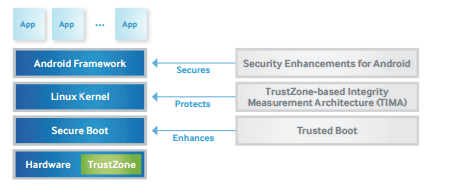
\includegraphics[scale=0.9]{Images/samsung_knox_platform_security}
\caption{Samsung Knox Platform Security}
\end{figure}
In der Grafik links sieht man den groben Aufbau eines Android Systems.In der Grafik rechts sieht man die Technologien, mit deren Hilfe es Samsung möglich ist in die Schichten einzugreifen.
\paragraph{Kerntechnologien der Platform Security}

\begin{itemize}
	\item \textbf{SE for Android}
	\begin{itemize}
		\item \textbf{Funktionsweise} \newline SE for Android basiert auf SELinux-Technologie und definiert die Zugriffskontrolle auf Linux-Ebene. Mandatory Access Control (MAC) und Discretionary Access Control (DAC) überwachen und verwalten welche Dateien und Apps auf das System des Geräts zugreifen können.
		\item \textbf{Sicherheit} \newline SE for Android erzwingt MAC, wobei Apps nur genau die Rechte zugewiesen erhalten, die sie für den Zugriff auf das System des Geräts benötigen. Sollte ein böswilliger Benutzer oder eine bösartige App also Zugriff auf das Gerät erhalten, dann betrifft der Schaden immer nur einen bestimmten Bereich, während die restlichen Bereiche des Geräts geschützt bleiben. \par Wenn SE for Android ausgelöst wird, sendet es eine Präventionsinformationsmeldung an den Benutzer des Geräts, die in der Informationsleiste erscheint. Die Präventionsinformationsmeldung gibt an, welche Anwendung versucht hat, auf Daten des Geräts zuzugreifen, und sie wird die Deinstallation der betreffenden Anwendung empfehlen. Beachten Sie dabei jedoch, dass SE for Android auch von autorisierten Anwendungen ausgelöst werden kann. Dies kann vorkommen, wenn die App einen von dem in der SE for Android-Richtlinie vorgegebenen Pfad verwendet. Wenn dies der Fall ist, sollten Sie die Datei der Sicherheitsrichtlinie entsprechend aktualisieren.
	\end{itemize}
	\item \textbf{ARM TrustZone-Based Integrity Measurement Architecture (TIMA)}
	\begin{itemize}
		\item \textbf{Funktionsweise} \newline TIMA schützt Ihr Gerät auf zwei verschiedene Weisen. Erstens prüft sie in regelmäßigen Abständen, ob der Kernel des Geräts geändert wurde, indem sie den gegenwärtigen Zustand mit dem Original-Kernel vergleicht. Zweitens authentifiziert TIMA Kernel-Module, wenn diese geladen werden, sodass Geräte nie ungeschützt sind.
		\item \textbf{Sicherheit} \newline Die TIMA TrustZone ist ein manipulationssicherer Sektor des ARM-Prozessors in Ihrem Gerät. Sie authentifiziert und verifiziert den Linux-Kernel über regelmäßige Messungen. Wenn TIMA for Android ausgelöst wird, sendet es eine Ermittlungsinformationsmeldung an den Benutzer, die in der Informationsleiste erscheint. In der Meldung werden Sie normalerweise zum Neustart des Geräts aufgefordert.
	\end{itemize}
	\item \textbf{Secure Boot und Trusted Boot}
	\begin{itemize}
		\item \textbf{Funktionsweise} \newline Secure Boot verhindert, dass unbefugte Bootloader und Kernels in das Gerät geladen werden. Dies bedeutet, dass Ihr Gerät nicht manipuliert wurde und der KNOX-Container geladen werden kann. \par Trusted Boot vergleicht den Bootloader und den Kernel des Betriebssystems mit den originalen Werksversionen. Dies wird dadurch erreicht, dass die Originaldaten des Geräts aufgezeichnet werden und das Gerät permanent beim Systemstart mit diesen gegengeprüft wird, um sicherzustellen, dass sich diese Daten nicht geändert haben.
		\item \textbf Sicherheit \newline Es gibt vier Bootloader auf dem Gerät. Jeder Bootloader prüft die Gültigkeit des vorhergehenden Bootloaders oder Kernels. Trusted Boot sichert diese Bootloader. Die Funktion ist in der ARM TrustZone, einem manipulationssicheren Sektor des ARM-Prozessors, eingebettet. Trusted Boot verwendet kryptografische Schlüssel, um sicherzustellen, dass die Messungen am Gerät dem Original entsprechen. Diese Schlüssel werden erst von Trusted Boot freigegeben, wenn SE for Android bestätigt, dass genehmigte Firmware auf dem Gerät ausgeführt wird.
	\end{itemize}
\end{itemize}

\subsubsection{Application Security}
\paragraph{Application Containers}
Container sind quasi ein Android im Android und bezeichnet einen gesicherten, separaten Bereich (Container) auf dem Gerät. Dieser Bereich hat einen eigenen Homescreen, eigene Anwendungen und eigene Daten. Diese Funktion ist damit vergleichbar mit einer Art Dual-Boot-Variante. Anwendungen außerhalb des Containers haben dabei keinerlei Zugriff auf die Daten oder Prozesse innerhalb des Containers. Anwendungen innerhalb des Containers haben grundsätzlich keinen Zugriff auf Daten außerhalb des Containers. 
\par 
Mittels Richtlinienkonfiguration kann der IT-Verwalter des Gerätes einen read-only (nur lesen) Zugriff für bestimmte Anwendungen im Container auf Daten außerhalb des Containers einrichten. Umgekehrt besteht diese Möglichkeit allerdings nicht. Daten innerhalb des Containers werden dabei mit einem Verschlüsselungsalgorithmus und einem AES-256 Bit Schlüssel geschützt. Ein Zugriff ist erst nach Eingabe eines Passwortes möglich.
\paragraph{On-Device Data Encryption (ODE)}
ODE ist ein im Knox enthaltenes Feature zur Verschlüsselung von Daten. Dabei kann sowohl der sichere Container als auch der normale Bereich, sowie interner als auch externer Speicher verschlüsselt werden. Verwendet wird ein AES Algorithmus mit einem 256 Bit starken Schlüssel. Die Verschlüsselungsfunktion kann vom User selbst unter den Einstellungen oder vom IT Administrator durch eine Richtlinie aktiviert werden.
\paragraph{Virtual Private Network (VPN) Support }
VPN-Verbindungen verwendet man um sicherzustellen, dass Daten bei der Übertragung geschützt sind und um den Netzwerkverkehr nicht mit den Daten von persönlichen Apps zu belasten.
\begin{itemize}
	\item \textbf{Funktionsweise} \newline 
	KNOX Workspace bietet 3 VPN-Optionen für den Schutz Ihrer Daten bei der Übertragung. Ein geräteweites VPN kann von Benutzern konfiguriert werden, sofern sie den entsprechenden Servernamen und die dazugehörigen Informationen zur Hand haben. VPN pro App oder ein containerweites VPN kann von IT-Administratoren über die MDM-Konsole eingerichtet werden. Auf der MDM-Konsole kann man bis zu 5 verschiedene VPN-Profile einrichten und diese einzelnen Apps zuweisen, um VPN pro App zu implementieren.
	\item \textbf{Sicherheit} \newline 
	VPN-Verbindungen sind die sicherste Methode, um die Daten bei der Übertragung zu schützen. Der KNOX VPN-Client kann ein bestehendes VPN-Gateway für den Schutz von Daten verwenden. KNOX VPN ist über Ihre MDM-Konsole im FIPS-Modus konfigurierbar. Zu den Sicherheitsfunktionen gehören NSA-Suite-B-Algorithmen, Unterstützung für X.509 mit Zertifikatsprüfung auf OCSP-Basis und 256-Bit-AES-Verschlüsselung. Wenn Ihr Unternehmen SmartCards verwendet, können diese mit VPN-Anmeldedaten konfiguriert werden.
\end{itemize}

\subsubsection{Management}
Mit MDM (Mobile Device Management) bietet Samsung Knox der IT Abteilung des Unternehmens die Möglichkeit eine integrierte Lösung zur Verwaltung und Administration von Samsung-Geräten vorzunehmen, ohne dabei auf Drittanbieter zurückgreifen zu müssen. Der Nachteil dabei ist die ausschließliche Verwendung mit Samsung-Geräten, welche über Samsung Knox verfügen.
\par
Samsung Knox gibt es in 2 Varianten, wobei beide Varianten ein MDM als Basis benötigen um zu funktionieren.
\paragraph{Knox Lösungen}
\begin{itemize}
	\item \textbf{Knox Express} \newline
	Diese Lösung ist für kleine bis mittelständische Unternehmen gedacht. Sie ist gratis, jedoch limitiert auf 250 Geräte. \par Falls die 250 Plätze nicht mehr reichen, kann man Knox Express problemlos auf Knox Premium updaten. \par Das ist die Variante, die die Projektgruppe empfehlen würde, da sie gratis ist und da laut Angaben von der Firma Kapsch es eher unwahrscheinlich ist, dass ein Kunde mehr als 250 Geräte hat und falls doch ist es ja problemlos auf Premium erweiterbar.
	\item \textbf{Knox Premium} \newline
	Diese Komplettlösung eignet sich ideal für Unternehmen, in denen Sicherheit oberste Priorität hat. \par Knox Premium kostet pro Gerät pro Monat 1\$ und kann um zusätzliche Add-ons erweitert werden. \par Weiters bietet Knox Premium einige zusätzliche Features für Android und eine bessere IOS Integration. In Hinblick auf die von Kapsch erwünschten Funktionalitäten bringen diese zusätzlichen Features jedoch keine Vorteile.
	\item \textbf{Add-Ons}
	\begin{itemize}
		\item \textbf{Knox Workspace} \newline
		Knox Workspace ist eine Erweiterung im Bereich Container. \par Dieses Add-on bietet eine einfachere Konfiguration, zwei Container pro Gerät, zusätzliche Apps und verbesserte Sicherheitsfunktionen. \par Die Hauptfeatures, die Workspace mit sich bringt, sind: 
		\begin{itemize}
			\item Erweiterte Containerverwaltung mit sicheren Richtlinien
			\item Datenverschlüsselung bei jedem Entsperren des Containers
			\item Pro-App-VPN für sichere und schnelle Verbindung
			\item Support für zwei separate Container für maximale Produktivität und für Trennung von arbeitsbezogenen und privaten Daten
		\end{itemize}
	All diese Einstellungen, die mit Knox Workspace dazu kommen, gelten nur innerhalb des Containers. Da es jedoch keine Einstellung gibt um zu verhindern, dass der Benutzer den Container verlässt und somit alle Workspace-Einstellungen umgeht, ist dieses Add-on in unserem Fall ungeeignet. \par Jedoch soll in Zukunft eine Art Contaier-only-mode implementiert werden. Sobald dieser vorhanden ist, wäre Knox Worspace auf jeden Fall ein Addon das in Betracht gezogen werden sollte.
		\item \textbf{Knox IAM\footnote{Identity and Access Management}} \newline
		Knox IAM ist eine SSO-Lösung(Single Sign-On-Lösung). \par Das heißt mit dem IAM Add-on hat man nur mehr einen einzigen Account, mit den man sich in allen Apps anmelden kann.
	\end{itemize}
\end{itemize}
\paragraph{MDMs}
Knox bietet zur Verwaltung der Geräte ein eigenes MDM, das EMM\footnote{Enterprise Marketing Management}, hat aber auch genügend Partner, deren MDMs Samsung Knox Funktionen implementiert haben. \par
Samsung Knox funktioniert also mit jedem MDM aus der nachfolgenden Liste:
\begin{itemize}
	\item \textbf{Liste an Kompatiblen MDMs}
	\begin{itemize}
		\item Samsung EMM
		\item MobileIron
		\item Absolute Software
		\item AirWatch
		\item CA Technologies
		\item Centrify
		\item Citrix
		\item FancyIron
		\item MaaS360
		\item NQ Mobile
		\item Samsung SDS
		\item SAP
		\item SOTI
	\end{itemize}
	\item \textbf{Samsung EMM} \newline
	Samsung KNOX EMM ist eine cloudbasierte Verwaltungslösung für Unternehmen. IT-Administratoren können damit Benutzer, Apps und plattformübergreifende Geräte über eine cloudbasierte Konsole verwalten. Außerdem bietet KNOX EMM Single Sign-On (SSO) und eine starke Authentifizierung für eine benutzerfreundliche und sichere Arbeitsumgebung für Mitarbeiter. \par Es ist einfach zu installieren und sehr übersichtlich gestaltet. Falls in der Firma noch keine andere MDM Lösung installiert sein sollte, ist EMM zu empfehlen.
\end{itemize}




